
% ===========================================================================
% Title:
% ---------------------------------------------------------------------------
% to create Type I fonts type "dvips -P cmz -t letter <filename>"
% ===========================================================================
\documentclass[11pt]{article}       %--- LATEX 2e base
\usepackage{latexsym}               %--- LATEX 2e base
\usepackage{tikz}
\usetikzlibrary{shapes.geometric, arrows}
\usepackage{booktabs}
\usepackage{graphicx}
%---------------- Tikz Flow D -----------------------------------------------

\tikzstyle{startstop} = [rectangle, rounded corners, minimum width=3cm, minimum height=1cm,text centered, draw=black, fill=red!30]
\tikzstyle{io} = [trapezium, trapezium left angle=70, trapezium right angle=110, minimum width=3cm, minimum height=1cm, text centered, draw=black, fill=blue!30]
\tikzstyle{process} = [rectangle, minimum width=3cm, minimum height=1cm, text centered, draw=black, fill=orange!30]
\tikzstyle{decision} = [diamond, minimum width=3cm, minimum height=1cm, text centered, draw=black, fill=green!30]
\tikzstyle{arrow} = [thick,->,>=stealth]

%---------------- Wide format -----------------------------------------------
\textwidth=6in \textheight=9in \oddsidemargin=0.25in
\evensidemargin=0.25in \topmargin=-0.5in
%--------------- Def., Theorem, Proof, etc. ---------------------------------
\newtheorem{definition}{Definition}
\newtheorem{theorem}{Theorem}
\newtheorem{lemma}{Lemma}
\newtheorem{corollary}{Corollary}
\newtheorem{property}{Property}
\newtheorem{observation}{Observation}
\newtheorem{fact}{Fact}
\usepackage{natbib}
\newenvironment{proof}           {\noindent{\bf Proof.} }%
                                 {\null\hfill$\Box$\par\medskip}
%--------------- Algorithm --------------------------------------------------
\newtheorem{algX}{Algorithm}
\newenvironment{algorithm}       {\begin{algX}\begin{em}}%
                                 {\par\noindent --- End of Algorithm ---
                                 \end{em}\end{algX}}
\newcommand{\step}[2]            {\begin{list}{}
                                  {  \setlength{\topsep}{0cm}
                                     \setlength{\partopsep}{0cm}
                                     \setlength{\leftmargin}{0.8cm}
                                     \setlength{\labelwidth}{0.7cm}
                                     \setlength{\labelsep}{0.1cm}    }
                                  \item[#1]#2    \end{list}}
                                 % usage: \begin{algorithm} \label{xyz}
                                 %        ... \step{(1)}{...} ...
                                 %        \end{algorithm}
%--------------- Figures ----------------------------------------------------
\usepackage{graphicx}

\newcommand{\includeFig}[3]      {\begin{figure}[htb] \begin{center}
                                 \includegraphics
                                 [width=4in,keepaspectratio] %comment this line to disable scaling
                                 {#2}\caption{\label{#1}#3} \end{center} \end{figure}}
                                 % usage: \includeFig{label}{file}{caption}


% ===========================================================================
\begin{document}
% ===========================================================================

% ############################################################################
% Title
% ############################################################################

\title{Parallel Genetic Algorithms on the GPU}


% ############################################################################
% Author(s) (no blank lines !)
\author{
% ############################################################################
George Savin\\
School of Computer Science\\
Carleton University\\
Ottawa, Canada K1S 5B6\\
{\em georgesavin@cmail.carleton.ca}
% ############################################################################
} % end-authors
% ############################################################################

\maketitle

% ############################################################################
% Abstract
% ############################################################################
\begin{abstract}
Genetic Algorithms are very powerful metaheuristics that have been successfully applied in 
various disparate fields. While there are many sequential parts to the algorithm, a fair amount
can and has been parallelized in MIMD and SIMD fashion. In this paper, we show a SIMD GPU solution to the the knapsack combinatorial problem. We do everything, including initialization of data on the device rather than the host CPU and show speed improvements across the board.
\end{abstract}

% ############################################################################
\section{Introduction} \label{intro}
% ############################################################################

Genetic algorithms are powerful metaheuristics that draw insipiration from evolutionary ideas. Through operations such as selection, cross-over and mutation, the solution space is "evolved" and more optimal results are found each iteration (generation). These algorithms are amenable to parallelization and indeed researchers have experimented with parallelizing everything from individual operators to the whole process. However, designing parallel algorithms can differ quite fundamentally given the underlying architecture. 
Empirical and experimental researchers have predominantly been the drivers of GAs, mainly as optimization tools. 
Only two main components for most GAs that are problem specific : encoding and evaluation.
Financial pattern discovery, MAX-3SAT, layout problems, ML hyperparameter selection \cite{} are but a few of the problems GPU GAs have been used to solve.

% ############################################################################
\section{Literature Review} \label{litrev}
% ############################################################################

Using GPUs to accelerate Genetic Algorithms started to take off when NVIDIA released CUDA SDK 2.0 in 2008, allowing for more general programming tasks to be parallelized.  

A first intuitive approach is to move an operator onto the GPU that can efficiently be ran in parallel, such as the fitness evaluation across a population \cite{Maitre2009-wd}. Taking this idea further, generation of chromosomes could also moved to the GPU \cite{Cavuoti2013-oy}. Unfortunately, this constant transfer between CPU and GPU at every generation slowed down the runtime, and depending on the population size, may not have even been worth it \cite{robilliard2008population}. 

To overcome this transfer slowdown, master-slave models of a binary and real coded GAs were completely ported to the GPU \cite{Debattisti2009-su, Arora2010-ds}. Each operator (tournament selection, two-point and single point crossover, bitwise XOR mutation) became separate CUDA kernels. Both the crossover and mutation kernels in these cases suffered from the possibility of having the same chromosome operated on many times, causing inefficient usage and propagation of sub-optimal solutions.

Because of the architectural and operational constraints of the GPU, such as limited shared memory and expensive global memory lookups, models that aimed to reduce global communication fared better. Inversely, these models seemed to have less overall accuracy \cite{Zheng2011-zr}, while other works found this difference non-existant \cite{jahne2016overview}. Further follow-ups to quality of solutions between models have not been explored.

Island model GAs divide populations in the hope that diversity is preserved during evolution. On a GPU, this roughly translates to thread blocks as islands, and single threads to individuals. Within a block, fast memory access and synchronisation is available. Migration between islands occurs asynchronously.
Early island model implementations \cite{Pospichal2010-lf, Van_Luong2010-mw} used global memory only for migration. They were applied to numerical and combinatorial optimisations problems with tremendous speed-ups recorded. These speed-ups unfortunately were due mainly to comparisons with poorly optimized sequential GAs \cite{Jaros2012-ni}. When compared against properly parallelized GAs on CPUs, the speed-up was more in line with expected theoretical analysis. A similar revision of speed-up was seen with newer master-slave implementations \cite{Sinha2015-dk}. Trade-offs between speed and solution quality were analyzed and associated to parameter tuning, specifically island, generation and chromosome counts \cite{Sun2019-fj}.

During this time, research looking at optimizing GA GPU representations as well as technique improvements to leverage more parallelization was taking off. Building on the island model implementations, simulated annealing was shown to provide faster convergence when replacing mutation \cite{li2017parallel}. Memory layouts were also explored, and chromosome based layouts proved to increase locality and make better usage of caches \cite{jahne2016overview}. Different encoding representations also increased convergence speed at no detriment to solution quality \cite{Pedemonte2011-zu}. 

Newer work incorporates some of these techniques, as well as developing new ones targeting Island models almost exclusively. Random seed improvement lead to a solution technique that only generates a single random seed, yet still benefits from the uniqueness and speed one would typically get by generating seeds every generation \cite{Sun2019-fj}. Another recent paper used the idea of synchronous migration intervals to improve solution quality by avoiding unintended migrations \cite{Janssen2022-kr}. This one in particular also used the idea of allocating multiple threads per individual \cite{shah2010gpu} combined with better data organization and found that their techniques provided up to 18x speedups and better solution quality compared to the original IMGAs on the same hardware.
Newer work tries to use warp granularity to represent each island and reduce thread divergence \cite{Amin2022-xd}. They also perform synchronous and asynchronous replacement, improving solution quality, dubbing it Two-Replacement Policy. Unfortunately, these interesting island model changes were not compared to any prior island model implementations.

% ############################################################################
\section{Problem Statement} \label{probstat}
% ############################################################################



% ############################################################################
\section{Background} \label{backg}
% ############################################################################

\subsection{Genetic Algorithms}
\subsection{GPU Programming}

% ############################################################################
\section{Proposed Solution} \label{propsol}
% ############################################################################
\subsection{CPU}

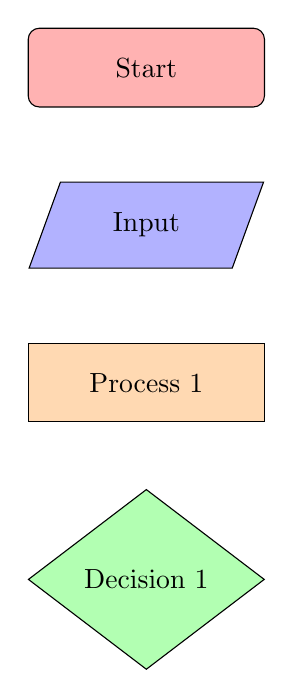
\begin{tikzpicture}[node distance=2cm]
\node (start) [startstop] {Start};
\node (in1) [io, below of=start] {Input};
\node (pro1) [process, below of=in1] {Process 1};
\node (dec1) [decision, below of=pro1, yshift=-0.5cm] {Decision 1};

\end{tikzpicture}


\subsection{GPU}


% ############################################################################
\section{Experimental Evaluation} \label{expeval}
% ############################################################################

\begin{table}[]
\centering
\resizebox{\textwidth}{!}{%
\begin{tabular}{@{}lllll@{}}
\toprule
Time (\%) & Total Time (ns) & Instances & Avg (ns)  & Name of Kernel          \\ \midrule
83.1      & 920,536,735     & 5,994     & 153,576.4 & GPUreproduceChromosomes \\
8.7       & 96,057,554      & 6,000     & 16,009.6  & evaluateChromosomes     \\
6.5       & 71,702,476      & 6,000     & 11,950.4  & pullScores              \\
1.4       & 15,998,624      & 6,000     & 2,666.4   & reduce                  \\
0.2       & 2,320,024       & 6         & 386,670.7 & initializeChromosomes   \\
0.1       & 1,613,520       & 6         & 268,920.0 & initKernel              \\ \bottomrule
\end{tabular}%
}
\caption{nsys profile of a 1000 generation GPU run}
\label{tab:gpu-profile}
\end{table}

\begin{table}[]
\begin{tabular}{@{}ll@{}}
\toprule
Call in Reproduction Kernel & Time (\%) \\ \midrule
Roulette Selection          & 12.2     \\
Crossover                   & 31.8     \\
Mutation                    & 56       \\ \bottomrule
\end{tabular}
\caption{The three device functions representing the majority of the work done in the reproduction kernel}
\label{tab:rep-kernel-breakdown}
\end{table}

% ############################################################################
\section{Conclusions} \label{conc}
% ############################################################################

% ############################################################################
% Bibliography
% ############################################################################
\bibliographystyle{plain}
\bibliography{my-bibliography}     %loads my-bibliography.bib

% ============================================================================
\end{document}
% ============================================================================
